%%
% Plantilla de reporte técnico para proyecto de listas enlazadas y sensores IoT
% Basado en plantilla IEEEtran
% Modificación: Diego Eduardo Zapata Aguilar - 30/OCT/2025
%
\documentclass[conference]{IEEEtran}

\usepackage[spanish]{babel}
\usepackage{amsmath,amssymb,amsfonts,amsthm}
\usepackage{graphicx}
\usepackage[utf8]{inputenc}
\usepackage{url}
\usepackage{hyperref}
\usepackage{subfig}
\usepackage{lipsum}
\usepackage{balance}
\usepackage{listings}
\usepackage{xcolor}

% Configuración de listings para código C++
\lstset{
    language=C++,
    basicstyle=\ttfamily\footnotesize,
    keywordstyle=\color{blue},
    commentstyle=\color{green!60!black},
    stringstyle=\color{red},
    numbers=left,
    numberstyle=\tiny\color{gray},
    breaklines=true,
    frame=single,
    showstringspaces=false
}

%%%%%%%%%%%%%%%%%%%%%%%%%%%%%%%%%%%%%%%%%%%%%
% PARCHE PARA ELIMINAR LA FECHA DEL DOCUMENTO
\usepackage{etoolbox}
\makeatletter
\patchcmd{\frontmatter@RRAP@format}{(}{}{}{}
\patchcmd{\frontmatter@RRAP@format}{)}{}{}{}
\makeatother	
%%%%%%%%%%%%%%%%%%%%%%%%%%%%%%%%%%%%%%%%%%%%%

\usepackage{datetime}
\newdateformat{specialdate}{\twodigit{\THEDAY}-\twodigit{\THEMONTH}-\THEYEAR}
\date{\specialdate\today}

\renewcommand\spanishtablename{Tabla}
\renewcommand\spanishfigurename{Figura}

\begin{document}

%%%%%%%%%%%%%%%%%%%%%%%%%%%%%%%%%%%%%%%%%%%%%
% Definitions
\newcommand{\breite}{1.0}
\newcommand{\RelacionFiguradoscolumnas}{0.9}
\newcommand{\RelacionFiguradoscolumnasPuntoCinco}{0.45}
%%%%%%%%%%%%%%%%%%%%%%%%%%%%%%%%%%%%%%%%%%%%%

% Title
\title{Sistema de Gestión Polimórfica de Sensores para IoT con Listas Enlazadas\\
\large Estructura de datos - Unidad 2}

% Author
\author{\IEEEauthorblockN{Junior Arturo Vazquez Leonel}
	\IEEEauthorblockA{Ingeniería en Tecnologías de la Información\\
		Universidad Politécnica de Victoria\\
		Semestre: Sep-Dic 2025}
}

\maketitle

\begin{abstract}
Este proyecto presenta la implementación de un sistema de gestión polimórfica de sensores IoT utilizando estructuras de datos dinámicas (listas enlazadas simples) en C++. El sistema integra sensores de temperatura y presión con comunicación serial a través de ESP32, demostrando conceptos fundamentales de programación orientada a objetos como herencia, polimorfismo y gestión dinámica de memoria sin el uso de contenedores STL. Se implementaron contenedores genéricos mediante plantillas (templates) para el almacenamiento eficiente de lecturas, y se desarrolló una interfaz de usuario interactiva por consola con seis opciones de gestión. El proyecto incluye documentación técnica completa generada con Doxygen, firmware ESP32 con PlatformIO y organización modular del código fuente.
\end{abstract}

\section{Introducción}

El Internet de las Cosas (IoT) ha transformado la manera en que los dispositivos interactúan y recopilan datos del entorno. En este contexto, el desarrollo de sistemas capaces de gestionar múltiples tipos de sensores de forma eficiente y escalable es fundamental para aplicaciones de monitoreo en tiempo real.

Este proyecto aborda el diseño e implementación de un sistema de gestión de sensores que aprovecha las características de la programación orientada a objetos para crear una arquitectura flexible y extensible. El uso de listas enlazadas simples implementadas manualmente (sin contenedores STL) permite la gestión dinámica de sensores sin limitaciones de tamaño predefinido, mientras que el polimorfismo facilita el procesamiento uniforme de diferentes tipos de sensores.

La comunicación con dispositivos ESP32 mediante el protocolo serial POSIX permite la adquisición de datos en tiempo real, simulando un entorno IoT real donde sensores distribuidos envían información de temperatura y presión. El sistema implementa un menú interactivo que permite crear sensores, registrar lecturas manualmente o desde ESP32, procesar datos de forma polimórfica y liberar recursos de manera segura.

\subsection{Objetivos}

\begin{itemize}
    \item Implementar estructuras de datos dinámicas (listas enlazadas simples) sin uso de STL
    \item Aplicar conceptos de herencia y polimorfismo con clases abstractas
    \item Desarrollar comunicación serial POSIX con ESP32 para adquisición de datos
    \item Demostrar el uso de plantillas (templates) para código genérico y reutilizable
    \item Implementar gestión manual de memoria con destructores en cascada
    \item Generar documentación técnica profesional mediante Doxygen con diagramas
    \item Desarrollar firmware ESP32 con PlatformIO para generación de datos
\end{itemize}

\section{Manual Técnico}

\subsection{Diseño del Sistema}

El sistema está diseñado siguiendo principios de programación orientada a objetos, con una arquitectura de tres capas:

\subsubsection{Capa de Abstracción de Sensores}

La clase base abstracta \texttt{SensorBase} define la interfaz común para todos los tipos de sensores:

\vspace{0.3cm}
\begin{lstlisting}
class SensorBase {
public:
    SensorBase(const char* nom);
    virtual ~SensorBase();
    virtual void procesarLectura() = 0;
    virtual void imprimirInfo() const = 0;
protected:
    char nombre[50];
};
\end{lstlisting}
\vspace{0.2cm}

Esta clase proporciona:
\begin{itemize}
    \item Métodos virtuales puros para garantizar implementación en clases derivadas
    \item Destructor virtual para correcta liberación de memoria polimórfica
    \item Encapsulamiento de datos comunes (nombre del sensor)
\end{itemize}

\subsubsection{Capa de Especialización}

Las clases concretas \texttt{SensorTemperatura} y \texttt{SensorPresion} heredan de \texttt{SensorBase} y especializan el comportamiento:

\begin{itemize}
    \item \textbf{SensorTemperatura}: Maneja lecturas tipo \texttt{float}, calcula promedios y elimina valores mínimos
    \item \textbf{SensorPresion}: Maneja lecturas tipo \texttt{int}, calcula estadísticas básicas
\end{itemize}

Cada sensor mantiene un historial de lecturas mediante la plantilla \texttt{ListaSensor<T>}.

\subsubsection{Capa de Gestión}

La clase \texttt{ListaGeneral} actúa como contenedor principal:

\vspace{0.3cm}
\begin{lstlisting}
class ListaGeneral {
private:
    struct NodoGeneral {
        SensorBase* sensor;
        NodoGeneral* siguiente;
    };
    NodoGeneral* cabeza;
public:
    void insertar(SensorBase* sensor);
    void procesarTodos();
    ~ListaGeneral();
};
\end{lstlisting}
\vspace{0.2cm}

Implementa operaciones de:
\begin{itemize}
    \item Inserción dinámica de sensores al final de la lista
    \item Recorrido polimórfico para procesamiento con \texttt{procesarLectura()}
    \item Liberación automática de memoria en cascada en el destructor
    \item Gestión de nodos específicos con \texttt{NodoGeneral}
\end{itemize}

\subsection{Componentes del Sistema}

\subsubsection{Estructuras de Datos}

\textbf{Nodo Genérico (\texttt{ListaSensor.h})}

Plantilla de nodo para listas enlazadas simples:

\vspace{0.3cm}
\begin{lstlisting}
template <typename T>
struct Nodo {
    T valor;
    Nodo<T>* siguiente;
    Nodo(const T& val) : valor(val), siguiente(nullptr) {}
};
\end{lstlisting}
\vspace{0.3cm}

\textbf{Lista de Sensores (\texttt{ListaSensor<T>})}

Implementación genérica con operaciones de:
\begin{itemize}
    \item Inserción al final: $O(n)$
    \item Búsqueda de mínimo con \texttt{eliminarMin()}: $O(n)$
    \item Cálculo de promedio: $O(n)$
    \item Obtención de tamaño: $O(1)$
    \item Especializada para \texttt{float} (temperatura) e \texttt{int} (presión)
\end{itemize}

\subsubsection{Comunicación Serial}

\textbf{Clase SerialReader}

Gestiona la comunicación POSIX con ESP32 mediante \texttt{termios.h} usando patrón PIMPL:

\begin{itemize}
    \item Configuración a 115200 baudios para ESP32
    \item Puerto serial: \texttt{/dev/ttyUSB0}
    \item Lectura línea por línea con timeout
    \item Estructura \texttt{Reading} con union para tipos múltiples
    \item Gestión automática de recursos (RAII) con clase interna \texttt{SerialImpl}
\end{itemize}

Protocolo de comunicación:

\vspace{0.2cm}
\begin{verbatim}
FORMATO: TIPO,VALOR\n
EJEMPLO: T,25.3    (Temperatura en float)
         P,1015    (Presion en int)
\end{verbatim}
\vspace{0.3cm}

\subsubsection{Firmware ESP32}

El firmware desarrollado con PlatformIO simula dos sensores:

\begin{table}[h]
\centering
\caption{Especificaciones de sensores simulados}
\label{tab:sensores}
\begin{tabular}{|l|l|l|l|}
\hline
\textbf{Tipo} & \textbf{Identificador} & \textbf{Rango} & \textbf{Tipo Dato} \\ \hline
Temperatura & T & 15.0-35.0°C & float \\ \hline
Presión & P & 980-1050 hPa & int \\ \hline
\end{tabular}
\end{table}

Características del firmware:
\begin{itemize}
    \item Plataforma: ESP32-DevKitC (esp32dev)
    \item Framework: Arduino
    \item Intervalo de transmisión: 2 segundos
    \item Generación de valores aleatorios con \texttt{random()}
\end{itemize}

\subsection{Desarrollo}

\subsubsection{Herramientas Utilizadas}

\begin{itemize}
    \item \textbf{Compilador}: GCC (C++17)
    \item \textbf{Sistema de Build}: CMake 3.16+
    \item \textbf{IDE}: CLion / Visual Studio Code
    \item \textbf{Documentación}: Doxygen 1.9.8 con Graphviz
    \item \textbf{Control de Versiones}: Git + GitHub
    \item \textbf{Hardware}: ESP32-DevKitC
    \item \textbf{Plataforma Embebida}: PlatformIO
    \item \textbf{Sistema Operativo}: Linux (Ubuntu/Arch)
\end{itemize}

\subsubsection{Estructura del Proyecto}

\vspace{0.2cm}
\begin{verbatim}
ds-u2-actividad-1-listasenlazadassimples/
|-- include/              # Archivos de encabezado (.h)
|   |-- SensorBase.h
|   |-- SensorTemperatura.h
|   |-- SensorPresion.h
|   |-- ListaSensor.h
|   |-- ListaGeneral.h
|   +-- SerialReader.h
|-- src/                  # Implementaciones (.cpp)
|   |-- SensorBase.cpp
|   |-- SensorTemperatura.cpp
|   |-- SensorPresion.cpp
|   |-- ListaGeneral.cpp
|   +-- SerialReader.cpp
|-- main.cpp              # Programa principal con menu
|-- cmake-build-debug/    # Ejecutables compilados
|-- firmware/             # Firmware ESP32
|   +-- esp32-arduino/    # Proyecto PlatformIO
|-- docs/                 # Documentacion Doxygen
|   |-- html/             # Documentacion web
|   |-- latex/            # Documentacion PDF
|   +-- Doxyfile          # Configuracion Doxygen
|-- reporte/              # Reporte LaTeX (este documento)
|-- CMakeLists.txt        # Configuracion CMake
|-- .gitignore            # Archivos ignorados por Git
+-- README.md             # Documentacion del proyecto
\end{verbatim}
\vspace{0.2cm}

\subsubsection{Proceso de Compilación}

\vspace{0.3cm}
\begin{lstlisting}[language=bash]
# Crear directorio de compilacion
mkdir -p build && cd build

# Configurar con CMake
cmake ..

# Compilar
cmake --build .

# Ejecutar (requiere ESP32 conectado en /dev/ttyUSB0)
./iot_polimorfico
\end{lstlisting}
\vspace{0.2cm}

\subsubsection{Compilación de Firmware ESP32}

\vspace{0.3cm}
\begin{lstlisting}[language=bash]
# Ir al directorio del firmware
cd firmware/esp32-arduino

# Compilar y subir al ESP32
pio run -t upload

# Monitorear salida serial
pio device monitor -b 115200
\end{lstlisting}
\vspace{0.2cm}

\subsubsection{Generación de Documentación}

\vspace{0.3cm}
\begin{lstlisting}[language=bash]
# Generar docs con Doxygen
cd docs
doxygen Doxyfile

# Abrir documentacion HTML
firefox docs/html/index.html

# Generar PDF desde LaTeX
cd docs/latex && make
\end{lstlisting}
\vspace{0.2cm}

\section{Implementación y Resultados}

\subsection{Interfaz de Usuario}

El sistema presenta un menú interactivo por consola con las siguientes opciones:

\begin{enumerate}
    \item Crear Sensor de Temperatura (float) - Solicita nombre del sensor
    \item Crear Sensor de Presión (int) - Solicita nombre del sensor
    \item Registrar Lectura Manual - Solicita nombre y valor
    \item Leer desde ESP32 - Lee datos desde puerto serial /dev/ttyUSB0
    \item Procesar Todos los Sensores - Ejecuta procesamiento polimórfico
    \item Cerrar Sistema - Libera memoria y termina ejecución
\end{enumerate}

Características adicionales:
\begin{itemize}
    \item Validación de nombres duplicados con clase auxiliar \texttt{RegistroSensores}
    \item Identificación automática de tipo de sensor por nombre
    \item Procesamiento diferenciado: temperatura elimina mínimo antes de promediar
    \item Mensajes informativos de creación y destrucción
\end{itemize}

% Figuras con capturas de pantalla del sistema
\begin{figure}[h]
    \centering
    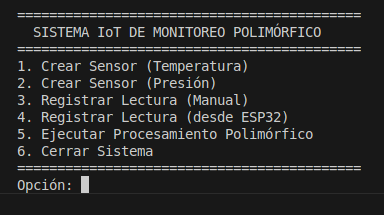
\includegraphics[width=\RelacionFiguradoscolumnas\columnwidth]{menu.png}
    \caption{Menú principal del sistema de gestión de sensores con las 6 opciones disponibles}
    \label{fig:menu}
\end{figure}

\begin{figure}[h]
    \centering
    \subfloat[Creación de sensor de temperatura]{
        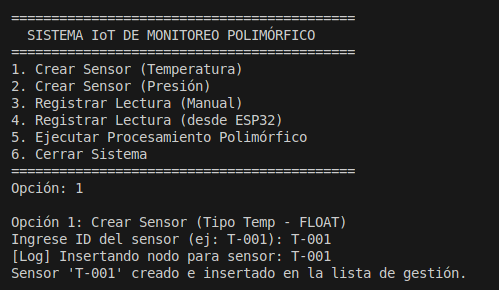
\includegraphics[width=\RelacionFiguradoscolumnasPuntoCinco\columnwidth]{crear_sensor_temperatura.png}
    }\hfill
    \subfloat[Creación de sensor de presión]{
        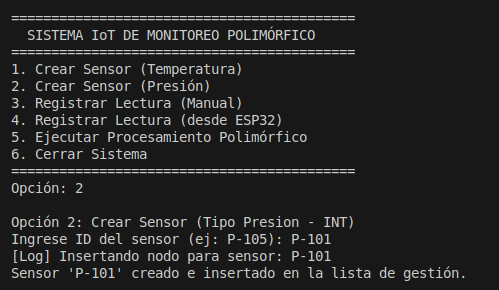
\includegraphics[width=\RelacionFiguradoscolumnasPuntoCinco\columnwidth]{crear_sensor_presion.png}
    }
    \caption{Proceso de creación de sensores de temperatura y presión (opciones 1 y 2)}
    \label{fig:creacion}
\end{figure}

\begin{figure}[h]
    \centering
    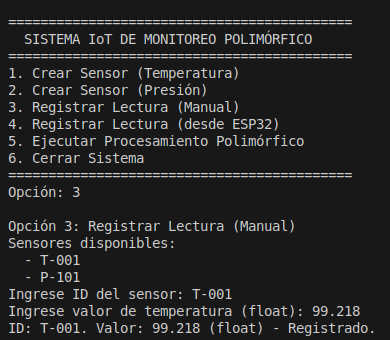
\includegraphics[width=\RelacionFiguradoscolumnas\columnwidth]{registrar_lectura_manual.png}
    \caption{Registro de lectura manual (opción 3)}
    \label{fig:lectura_manual}
\end{figure}

\begin{figure}[h]
    \centering
    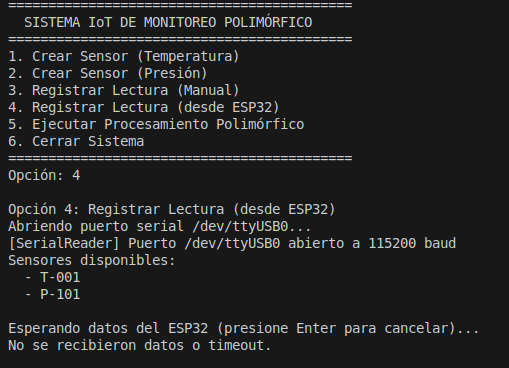
\includegraphics[width=\RelacionFiguradoscolumnas\columnwidth]{registro_lectura_ESP32.png}
    \caption{Adquisición de datos desde ESP32 vía puerto serial /dev/ttyUSB0 a 115200 baudios (opción 4)}
    \label{fig:arduino}
\end{figure}

\begin{figure}[h]
    \centering
    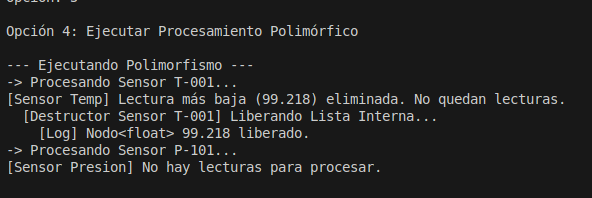
\includegraphics[width=\RelacionFiguradoscolumnas\columnwidth]{procesamiento_polimorfico.png}
    \caption{Ejecución del procesamiento polimórfico: temperatura elimina mínimo, presión calcula promedio directo (opción 5)}
    \label{fig:procesamiento}
\end{figure}

\begin{figure}[h]
    \centering
    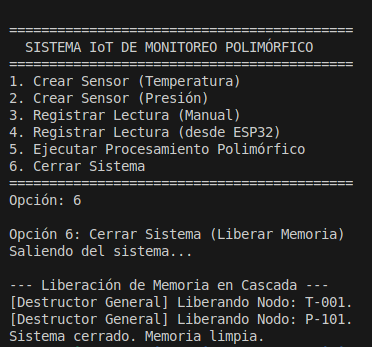
\includegraphics[width=\RelacionFiguradoscolumnas\columnwidth]{liberar_memoria.png}
    \caption{Liberación de memoria en cascada al cerrar el sistema (opción 6)}
    \label{fig:destruccion}
\end{figure}

\subsection{Validación de Funcionalidad}

El sistema fue validado mediante:

\begin{itemize}
    \item \textbf{Pruebas de compilación}: Compilación exitosa sin errores ni warnings
    \item \textbf{Pruebas de comunicación}: Correcta recepción de datos desde ESP32
    \item \textbf{Pruebas de polimorfismo}: Procesamiento diferenciado por tipo de sensor
    \item \textbf{Pruebas de robustez}: Manejo de nombres duplicados y valores inválidos
    \item \textbf{Pruebas de memoria}: Liberación correcta en cascada al cerrar sistema
    \item \textbf{Pruebas de listas}: Operaciones de inserción, búsqueda de mínimo y promedio
\end{itemize}

\subsection{Algoritmos Implementados}

\textbf{Procesamiento de Temperatura}
\begin{enumerate}
    \item Si hay 3 o más lecturas, eliminar el valor mínimo
    \item Calcular promedio de valores restantes
    \item Imprimir resultado en consola
\end{enumerate}

\textbf{Procesamiento de Presión}
\begin{enumerate}
    \item Calcular promedio directo de todas las lecturas
    \item Imprimir resultado en consola
\end{enumerate}

\subsection{Documentación Generada}

La documentación Doxygen incluye:

\begin{itemize}
    \item Jerarquía de clases con diagramas de herencia (SensorBase → Derivadas)
    \item Diagramas de colaboración y dependencias entre clases
    \item Gráficos de llamadas (call graphs) y llamantes (caller graphs)
    \item Documentación de cada método con parámetros y valores de retorno
    \item Documentación de estructuras internas (Nodo, NodoGeneral, Reading)
    \item Índice alfabético de símbolos y archivos
    \item Código fuente navegable con resaltado de sintaxis
    \item Formato HTML navegable y LaTeX para PDF
\end{itemize}

\section{Conclusiones}

Se logró implementar exitosamente un sistema de gestión polimórfica de sensores IoT que demuestra:

\begin{enumerate}
    \item \textbf{Estructuras dinámicas sin STL}: Las listas enlazadas implementadas manualmente permiten gestión flexible sin límites predefinidos y control total sobre la memoria
    \item \textbf{Polimorfismo efectivo}: El procesamiento uniforme de diferentes tipos de sensores mediante interfaces abstractas (\texttt{SensorBase}) y método virtual \texttt{procesarLectura()}
    \item \textbf{Plantillas genéricas}: El código reutilizable con \texttt{ListaSensor<T>} para diferentes tipos de datos (float e int)
    \item \textbf{Comunicación serial robusta}: Integración efectiva con hardware ESP32 mediante protocolo POSIX a 115200 baudios
    \item \textbf{Gestión manual de memoria}: Destructores en cascada y patrón RAII garantizan liberación correcta de recursos
    \item \textbf{Documentación completa}: Doxygen con diagramas, call graphs y código fuente documentado
\end{enumerate}